\cotefile{67}
\scanpage{53}
% slanted
\margin{torseurs sous groupe \unsure{diédrique|orthogonal|toriques} $\longleftrightarrow$ \deleted{(\unsure{symétrie, 1 tourne} $\unsure{\mathbb U/\mathbb Z_{2}}$, \unsure{à 2 élém.|const. échec})}}

\diagram{\begin{tikzcd}[ampersand replacement=\&,column sep=small,row sep=1em]
\text{Cercles toriques} \arrow[r,leftrightarrow] \&
\substack{\text{\deleted{\unsure{espace}} plan vectoriel \inserted{réel}}\\ \text{euclidien \deleted{\unsure{orié}}}} \arrow[r,leftrightarrow] \&
\left[\substack{\text{Droites vectorielles \inserted{unitaires} sur corps }C\\\text{iso. à }\mathbb C\ \text{(mais pas can. !)}}\right]\\
\substack{\text{Cercles toriques}\\\text{orientés}} \arrow[r,leftrightarrow] \arrow[d,leftrightarrow] \&
\substack{\text{\deleted{\unsure{espaces}} plans vectoriel}\\\text{réel orienté}} \arrow[r,leftrightarrow] \&
\substack{\text{\deleted{plans} \inserted{droites vectorielles} complexes }\deleted{\unsure{D}}\,T\\
\text{\deleted{structure \unsure{euclidienne}} \inserted{unitaires}}\\
\text{i.e. \deleted{avec} iso } T\simeq\overline{T^\vee}\\
T^\vee\simeq\overline T\ \text{i.e.}}\\
\text{torseurs sous }\mathbb U \arrow[rr,leftrightarrow] \& \&
\substack{\text{droites vectorielles complexes}\\ \text{conformes, avec \deleted{\unsure{disques}} jauge}\\
\text{\deleted{conformes} \deleted{\unsure{vectoriels}} conforme fixée }D}
\end{tikzcd}}

\deleted{\unsure{Le degré|Le topos|Le groupe} des objets des catégories}

\deleted{Soit $C', C''$ deux cercles toriques orientés, \unsure{alors} on a
$\operatorname{Isom}(C'^{-1},C'')\simeq\operatorname{Isom}(C''^{-1},C')$}

% slanted
\margin{anti-isom. des $\mathbb R^{*+}$-torseurs}

\uline{NB} Pour $D$ droite complexe fixée, on a Ens des jauges sur $D$
$=D^{\unsure{*|\times}}/\mathbb U$, et $J(D)\simeq J(D^\vee)_{\unsure{\varepsilon}}$ (car \(=\) groupe de rotations $\mathbb U_{\varepsilon}$).

Le passage au cercle torique \inserted{orienté} dual correspond au passage à l'espace vectoriel \deleted{\unsure{réel}} \deleted{\unsure{euclidien}} \inserted{complexe dual} $\deleted{\unsure{T}}T^\vee$ ($\simeq\overline T$)

La donnée, pour deux \deleted{\unsure{espaces}} \inserted{droites} vect complexes $T',T''$, d'un système $((D',D''),u)$, où $D',D''$ sont des jauges des $T',T''$ et $u\in\partial D'\mathbin{\wedge}_{\mathbb U}\partial D''$.
\[
\begin{aligned}
(&\simeq\operatorname{Isom}_{\mathbb U}\,\partial D'^{-1},\partial D''\\
 &\simeq\operatorname{Isom}_{\mathbb U}(\partial D''^{-1},\partial D')
 \simeq\operatorname{Isom}(T'^{-1},T'')\simeq\operatorname{Isom}(T''^{-1},T')\simeq\mathrm{Bases}(T'\otimes T'')\\
 &\simeq T'^{*}\mathbin{\wedge}_{\mathbb C^{*}}T''^{*}\}\simeq
 \deleted{\unsure{f\ ;D',D''\ ;\ \text{non}}}\ \text{dualités entre }(T',T'')\ )
\end{aligned}
\]
revient à la donnée d'un $v\in(T'\otimes_{C}T'')^{*}$ i.e. une dualité entre $T',T''$, \uline{plus} une jauge \inserted{$D'$} dans $T'$ (ou ce qui revient au $=$ \unsure{grâce à|grâce} \unsure{v}, plus une jauge $D''$ dans $T''$)
% archive sheet number: 55

\scanpage{54}
\mspage{1}

\uline{\unsure{11 1.84|11 I.84}}

\uline{Chirurgie conforme}

\textcircled{\unsure{4|A|1}} Surface conforme à bord. On \deleted{prend des} la définit par des cartes locales qui, au voisinage d'un point du bord, sont modelées sur \inserted{$\overline H=$} $(\Im z\geq 0)\subset\mathbb C$. Dans le cas $X$ orienté i.e structure holomorphe, la structure peut \deleted{\unsure{se|de}} définir par un faisceau de $\mathbb C$-algèbres, qui, sur le modèle $\overline H$ précédent, aux points $x$ de $\partial\overline H=\mathbb R$, est formée de germes de fonctions qui se \uline{prolongent} \deleted{\unsure{alors|des}} fonctions hol. \deleted{aux pts de} \inserted{au voisinage} de $x$ \uline{dans} $C$.

À ne pas confondre avec le sous faisceau plus grand du faisceau des fonctions complexes continues, savoir \deleted{celui des} \inserted{le f. des} fonctions continues qui sont hol dans $\operatorname{Int}(X)$.

\uline{Théorème 1} La structure conforme de $X$ (surface conforme à bord) est connue quand on la connaît dans $\operatorname{Int}(X)$, (ce qui suffit à déterminer le faisceau des fonctions \inserted{complexes} continues qui sont conformes dans $\operatorname{Int}(X)$).

Il suffit de voir que \unsure{cel|cela} permet de réconstituer les \uline{cartes} conformes des voisinages des points du bord. Je dis que ces cartes
% archive sheet number: 56

\scanpage{55}

$U\longrightarrow\overline H^{+}$ sont exactement les cartes topologiques (i.e. \deleted{applications continues injectives}, \inserted{plongements \deleted{inj.} \deleted{\unsure{de}} \inserted{ouverts}, ou encore \unsure{continues inj.|cartes au sens top.|continus inj.}} appliquant bord dans bord) qui sont conformes dans $\operatorname{Int}U$. Cela \deleted{\unsure{provient du|résulte du|précédent du}} \inserted{équivaut au}

\uline{Lemme 1} Soit $U$ un ouvert de $\overline H^{+}$, alors \deleted{toute} \deleted{application \inserted{\deleted{\unsure{continue}}} injective} plongement ouvert $f:U\longrightarrow\overline H$ \deleted{fonction continue sur $V$,} qui est holo dans $U\cap H$, est holo (i.e. se prolonge holomorphiquement dans $\mathbb C$, au voisinage de tt pt de $U\cap\partial H=U\cap\mathbb R$).

C'est un cas particulier du \uline{lemme de \unsure{Schwartz|Schwarz}}, qui dit que tte fonction \deleted{holo} continue complexe $f$ dans $U$, qui est \uline{réelle} sur $U\cap\mathbb R$, est holomorphe.

Pour terminer la dém du \deleted{lemme} \inserted{th}, il faut voir encore que le $f$ du lemme est bien (au voisinage de tt pt $x$ de $U\cap\partial H$) une carte holomorphe de $\deleted{\unsure{H|B|\partial}}U$ (i.e. de $H$) en $x$, i.e. que le germe \inserted{en $x$} de fonction holomorphe \uline{sur $\mathbb C$} défini par $f$ est inversible. Mais \deleted{\unsure{il}} ce germe n'est pas constant, \deleted{et la structure} \inserted{de par son} développement
% archive sheet number: 57

\scanpage{56}
\mspage{2}

en série qui commence par
\[
a_n z^n\text{ ---}\qquad n>0,\ a_n\ne0\qquad(\mathrm{OPS}\ x=0)
\]
on voit tout de suite que l'on doit avoir $n=1$ ---

% slanted
\margin{Noter : \uline{indétermination} d'une carte loc. au bord : modulo chgt. de coordonnées par un germe de fonction analytique \uuline{réelle}.}

[\uline{Thm 2} Équiv. de la cat. des surfaces conformes à bord \inserted{compactes,} avec celle des courbes alg. propres lisses sur $\mathbb R$.]

% slanted
\margin{\uline{NB} À partir d'ici $H$ désigne le demi-plan \uline{fermé} $\{z\in\mathbb C\mid\Im z\geq 0\}$}

\textcircled{\unsure{2|b}} \unsure{Découpe|Découpage} d'une surface conforme à bord, suivant un 1-complexe top. $K\subset X$, satisfaisant des hypothèses de régularité convenables (rectifiabilité suffit ?).

\uline{Théorème 3} La découpe $\widetilde X$, munie du \deleted{la} \deleted{structure} \inserted{faisceau} ``des fonctions \inserted{complexes} continues conformes dans $\operatorname{Int}(\tilde{\unsure{x|X}})$ ($\simeq X\smallsetminus K$), ``est'' une surface conforme à bord.

% slanted
\margin{C'est un th. du type ``uniformisation \deleted{\unsure{généralisée}} \inserted{à bord}''}

Cela revient à vérifier \deleted{deux} que \inserted{pour} tout point $\tilde x$ de $\partial\widetilde X$, il existe un voisinage \inserted{ouvert} $U$ de $x$, et un \deleted{\unsure{isom}} \inserted{homéo} de $U$ avec $H\cap\mathring{\mathbb D}$ (où $\mathbb D=\{z\in\mathbb C\mid |z|\leq 1\}$ est le disque unité de $\mathbb C$).

% slanted
\margin{\unsure{purement|revient} dans a) Cor. au thm.}

\figure{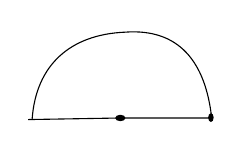
\begin{tikzpicture}[x=1cm,y=1cm]
\draw (0,0) .. controls (0.05,0.68) and (0.48,1.07) .. (1.18,1.10) .. controls (1.86,1.15) and (2.20,0.73) .. (2.28,0.01);
\draw (-0.05,-0.01) -- (1.12,0.01) -- (2.29,0.01);
\fill (1.12,0.01) ellipse (0.065 and 0.041);
\fill (2.27,0.015) ellipse (0.035 and 0.056);
\end{tikzpicture}}

Cela revient à deux choses, suivant que $x$ correspond :
% archive sheet number: 58

\scanpage{57}

un pt de $K$ d'ordre $\geq2$, ou d'ordre 1 :

\uline{Lemme} 2 Soi\deleted{\unsure{en}}t $K$ un segment topologique $\subset\mathbb C$, et $x\in K$. \inserted{On suppose $K$ assez régulier (rectifiable suffit ??).} Alors

a) Si $x$ n'est pas extrémité de $K$, alors il existe

\figure{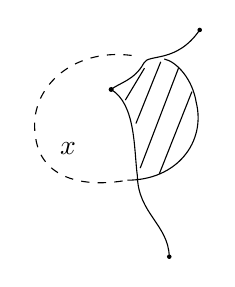
\begin{tikzpicture}[x=0.9cm,y=0.9cm]
\draw[dashed] (0.16,1.02) .. controls (-0.68,1.13) and (-1.30,0.55) .. (-1.20,-0.10) .. controls (-1.15,-0.65) and (-0.63,-0.87) .. (0.10,-0.74);
\draw (0.10,-0.74) .. controls (0.80,-0.74) and (1.21,-0.20) .. (1.07,0.36) .. controls (1.02,0.68) and (0.80,0.93) .. (0.62,0.97);
\draw (1.12,1.38) .. controls (0.79,0.90) and (0.39,1.05) .. (0.33,0.91) .. controls (0.20,0.67) and (-0.02,0.63) .. (-0.13,0.54) .. controls (0.22,0.33) and (0.19,-0.30) .. (0.24,-0.68) .. controls (0.25,-1.21) and (0.68,-1.37) .. (0.69,-1.82);
\draw (0.07,0.39)--(0.34,0.84) (0.22,0.06)--(0.57,0.93) (0.28,-0.57)--(0.82,0.84) (0.55,-0.65)--(1.01,0.51);
\fill (1.12,1.38) circle (.032) (-0.13,.54) circle (.035) (.69,-1.82) circle (.032);
\node at (-.74,-.29) {$x$};
\end{tikzpicture}}

\deleted{un voisinage \inserted{ouvert} $U$ de $x$ dans $\mathbb C$, ne contenant pas d'\unsure{extrémité|extrémités} de $U$, tel que $U\smallsetminus K\cap U$ ait deux composantes connexes $U'$ et $U''$ avec $\overline{U'}\cap U=U'\cup(K\cap U)$, $\overline{U''}\cap U=U''\cup(K\cap U)$, et \unsure{une|qu'une} fonction holo} application continue injective \deleted{de $\unsure{\mathbb D^\circ}$} $H\cap\mathbb D^\circ\longrightarrow\mathbb C$, \deleted{de $H\cap\mathring{\mathbb D}$ dans $\mathbb C$, hol. dans $H\cap\mathring{\mathbb D}$ dans $\mathbb C$, continue} holomorphe dans \deleted{$\mathbb D\smallsetminus\mathbb D\cap\mathbb R$} \inserted{$(\operatorname{Int}H)\cap\mathbb D^\circ$}, \deleted{$=\,]-1,+1[\,=(\unsure{\partial}\mathbb D^{++}\amalg D^{--})$ (mais pas néc\textsuperscript{t} aux deux pts de $\mathbb R$)} (mais pas néc hol. \deleted{dans} aux pts de $\partial H\cap\mathbb D^\circ=\,]-1,+1[$) telle que $f(\partial H\cap\mathbb D^\circ)\subset K$ et $f(0)=x$. De plus, pour une rive donnée de $K$ en $x$, OPS que ladite rive est celle déterminée par \inserted{$\operatorname{Im} f=$} $f(H\cap\mathbb D^\circ)$.

b) Si $x$ est extrémité de $K$, alors $\exists$ $f:H\cap\mathbb D^\circ\longrightarrow\mathbb C$, hol. \inserted{\deleted{et régulière}} dans $(\operatorname{Int}H)\cap\mathbb D^\circ$, \deleted{et injective dans $\unsure{\overline I|I}$ telle que $\unsure{f(-1)=f(1)|f(-t)=f(t)}$ \deleted{\unsure{(sinon)}} soit \unsure{avec} $f:$ telle que $f(0)=0$, $f(]-1,0)$ $f\mid ]-1,0]$ et $f\mid [0,1[$ soient injectifs,}

\figure{\begin{tikzpicture}[x=.8cm,y=.8cm]
\draw[dashed,dash pattern=on 9pt off 4pt] (0.18,1.06) .. controls (-.64,1.14) and (-1.22,.52) .. (-1.18,-.20) .. controls (-1.02,-.96) and (-.45,-1.36) .. (.12,-1.23) .. controls (.94,-1.05) and (1.20,-.28) .. (.98,.54);
\draw (.42,3.13) .. controls (.21,2.41) and (.56,1.78) .. (.28,1.28) .. controls (-.04,.83) and (-.22,.86) .. (.04,.25);
\fill (.04,.25) circle (.027);
\node at (0,-.12) {$x$};
\end{tikzpicture}}
% archive sheet number: 59

\scanpage{58}
\mspage{3}

et telle que

a) $f\mid(\operatorname{Int}H)\cap\mathbb D^\circ$ est injective, son image $\subset\mathbb C\smallsetminus K$

b) $f(0)=x$, \deleted{$\unsure{f(-1)=f(|f(\pm1)=f(|f(-t)=f(}$}

c) $f\mid ]-1,0]$ et $f\mid[0,1[$ injectives, avec même image $\subset K$.

\uline{Scholie} Chaque rive de $K$ \deleted{\unsure{est un}} \inserted{munit} $K$ d'une structure analytique réelle canonique, via l'inclusion de $K$ dans $\mathbb C$ (ou dans une surface conforme \unsure{qconle|qconque|quelle}), mais le passage de l'une à l'autre se fait par une application (identique) qui n'est pas un iso analytique : les \deleted{\unsure{parti}}propriétés de régularité (\deleted{\unsure{ca}}caractère $C^\infty$, ou analytique réel etc) reflètent sans doute les propriétés de régularité correspondantes de $K$ dans $\mathbb C$.

(Ceci \inserted{devrait} se \unsure{magnifier|manifester} dans \deleted{\unsure{le thm|le th.}} \inserted{un} Scholie plus circonstancié au théorème suivant).

\textcircled{3} \uline{Recollement}. On doit avoir un théorème dans le style du
% archive sheet number: 60

\scanpage{59}

\uline{Th. 4} Équivalence de catégories entre

a) Cat. des couples $(X,K,S)$ $X$ surface conforme à bord compacte, $(K,S)$ complexe top. \inserted{cpact} \deleted{\unsure{et|de|ext}} avec $\partial X\subset K\subset X$, $K$ assez régulier (rectifiable suffit)

% slanted
\margin{\uline{NB} On ne suppose pas les \unsure{cptes.|comp.|cpts.} conn. de $K\smallsetminus S$ des intervalles (il peut y avoir des cercles)}

b) Cat des systèmes $(\widetilde X,\widetilde S,\sigma)$, où $\widetilde X$ est une surface conforme à bord \inserted{compacte}, $\widetilde S$ une partie finie de $\partial\widetilde X$, $\sigma$ une involution de $\operatorname{Déc}(\partial\widetilde X/\widetilde S)$, $\sigma$ assez régulière (rectifiable suffit).

Le foncteur a) $\longrightarrow$ b) résulte du th. \unsure{3|1}, avec un complément qui explicite les propriétés de régularité de la fonction-recollement dont il a été question dans le lemme 2. Pour le foncteur en sens inverse, il est connu topologiquement, et comme faisceau structural conforme (large) sur $X$\inserted{$=\widetilde X/\unsure{\mathcal R|R}$}, on prend les fonctions continues qui sont conformes dans $X\smallsetminus K\simeq\operatorname{Int}\widetilde X$.
% archive sheet number: 61

\scanpage{60}
\mspage{\deleted{\unsure{3|5}} 4}

Le fait que ça donne bien une structure conforme à bord \deleted{équivaut} (qui automatiquement, \unsure{redonnera|redonne} \deleted{naissance} \inserted{avec $K$} à la structure conforme à bord $\widetilde X$ de départ) équivaut aux \deleted{lemme suivant :} \inserted{deux cas particuliers suivants}

\deleted{\uline{Lemme 3}

a) Soit $\sigma$ un homéomorphisme rectifiable (ou plus régulier que ça ?) de $[0,1]$ sur lui \deleted{\unsure{ou|même}}, avec $\sigma(0)=0$, $\sigma(1)=1$, alors il existe une \deleted{courbe} \inserted{partie fermée} $K\subset H\cap\mathbb D^\circ$, \deleted{bornée contenant 0, telle que $K\smallsetminus\{0\}$ soit contenue dans $\operatorname{Int} H$} \inserted{avec $K\cap\partial H=\{0\}$}, $K$ étant un intervalle demi-ouvert d'extrémité 0, qui partage $H\cap\mathbb D^\circ$ en deux comp. connexes $U',U''$. De plus, on trouve un

\figure{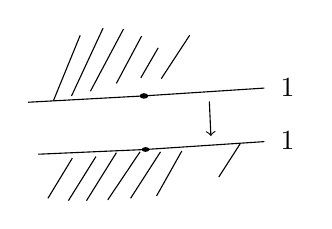
\begin{tikzpicture}[x=1cm,y=1cm]
\draw (0,1.0)--(1.46,1.08)--(3.0,1.18) (.13,.34)--(1.49,.40)--(3.00,.50);
\draw (.32,1.02)--(.66,1.85) (.55,1.08)--(.95,1.94) (.79,1.14)--(1.21,1.93) (1.12,1.24)--(1.44,1.84) (1.43,1.31)--(1.65,1.69) (1.69,1.30)--(2.05,1.85);
\draw (.56,.29)--(.25,-.22) (.86,.31)--(.51,-.25) (1.12,.36)--(.74,-.25) (1.42,.37)--(1.01,-.24) (1.68,.37)--(1.30,-.22) (1.95,.38)--(1.63,-.19) (2.69,.47)--(2.42,.05);
\draw[->] (2.30,1.01)--(2.32,.57);
\fill (1.47,1.08) ellipse (.055 and .035); \fill (1.49,.40) ellipse (.05 and .03);
\node[right] at (3.08,1.19) {$1$}; \node[right] at (3.08,.51) {$1$};
\end{tikzpicture}}

\figure{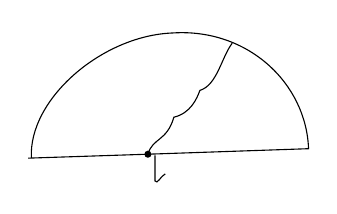
\begin{tikzpicture}[x=1cm,y=1cm]
\draw (0,0) .. controls (-.04,.75) and (.90,1.56) .. (1.80,1.59) .. controls (2.75,1.65) and (3.49,.95) .. (3.52,.12) -- (1.48,.05) -- (-.04,0);
\draw (1.48,.05) .. controls (1.54,.26) and (1.72,.21) .. (1.81,.52) .. controls (2.02,.57) and (2.10,.75) .. (2.14,.86) .. controls (2.36,.93) and (2.41,1.27) .. (2.55,1.46);
\fill (1.48,.05) circle (.045); \draw (1.57,.035)--(1.57,-.29) .. controls (1.60,-.34) and (1.64,-.23) .. (1.70,-.20);
\end{tikzpicture}}}

\uline{Lemme 3} Cas particuliers

a) Recollement de $H$ à $H$ \inserted{(\uline{deux exemplaires})} suivant un iso. rectifiable $[0,1]\overset{\sigma}{\longrightarrow}[0,1]$, regardé au voisinage de 0 [ou variante (\deleted{\unsure{mieux}} alors utiliser th. 3) : suivant un isom rectifiable $[-1,1]\overset{\sigma}{\longrightarrow}[-1,1]$, regardé au voisinage de 0].
% archive sheet number: 62

\scanpage{61}
\mspage{\deleted{\unsure{4|3}}}

b) Recollement de $\overline H$ à lui $=$ suivant un isom. rectifiable $[0,1]\overset{\sigma}{\longrightarrow}[-1,0]$ \inserted{$(\sigma(0)=0)$}, regardé au voisinage du pt 0.

% slanted
\margin{\uline{12.1} \deleted{\unsure{b)|a)}} c) Soit $C$ une courbe rectifiable dans \deleted{\unsure{le plan|disque}, \unsure{au bord}} \inserted{un ouvert $U$ de $\mathbb C$}, $f$ une \deleted{\unsure{germe de}} fonction complexe continue sur $U$ \deleted{\unsure{au v}} qui est continue dans $U\smallsetminus C$, alors $f$ est holomorphe dans $U$}

\textcircled{4} \uline{Recollements \deleted{bord à bord} \inserted{de disques}}. \inserted{Le recollement ``bord à bord''} Cela correspond, dans le th. 4, au cas où $K$ est une variété \inserted{(compacte)} de dim 1, $S=\varnothing$. \deleted{Il} Pour avoir ``des \unsure{nbs|ets} finis de modules'', il est naturel de dégager des conditions restrictives naturelles sur l'involution $\sigma$ \deleted{\unsure{de}} sur $\partial\widetilde X$.

Pour ceci, \deleted{rapp} on se rappelle que pour une surface conforme à bord $X$ \inserted{(au lieu de $\widetilde X$)} et une comp. connexe du bord, soit $C$, il revient au $=$ de se donner une structure de droite projective \inserted{(rectifiable)} sur $C$, ou un ``bouchage de trou'' en $C$ par un disque \inserted{de bord $C$} ; les propriétés de régularité (p.r. à la structure analytique réelle de $C$) de la structure de droite projective, reflètent
% archive sheet number: 63

\scanpage{62}
\mspage{5}

les propriétés de régularité de $C$ en tant que cercle \inserted{``intérieur''} dans la surface \deleted{\unsure{sans bord}} \inserted{conforme} $X'$ déduite par bouchage du trou. D'autre part, le choix d'un point de $D\smallsetminus C$ équivaut à celui d'une structure torique sur $C$ compatible avec la structure de droite projective réelle (i.e. une restriction du groupe structural \inserted{$\unsure{\mathrm{GP}(1,\mathbb R)|\mathrm{Gp}(1,\mathbb R)}=$} $\mathrm{Gl}(2,\mathbb R)/\mathbb R^{*}$ au sous-groupe cpct maximal $\mathrm O(2)/\pm1$).
--- et cel équivaut aussi à la donnée d'une structure \deleted{\unsure{do}}torique de $D$ sur \inserted{\unsure{la base|le bord}} $\partial D=C$. Notons que l'on aura alors une inclusion canonique
\[
D\subset T_{X',a}
\]
où $a$ est le centre choisi de $D$. On va expliciter \deleted{ainsi} ces dernières relations ainsi

\uline{Prop.} Équivalence entre \deleted{la cat. des surfaces \unsure{confo|conf.}}
% archive sheet number: 64

\scanpage{63}
% archive sheet number: 65

a) Cat. des surfaces conformes à bord $X$, avec comp. connexe \inserted{compacte} choisie $C$ du bord, et une structure toroïdale dessus rectifiable (?) pour sa structure analytique réelle, et

b) Cat. des surfaces conformes à bord \inserted{$X'$}, avec \deleted{\unsure{$D$|$H$|un}} disque pointé $(D,a)$, $D\subset\mathrm{Int}(X')$ marqué, tel que $\partial D$ soit rectifiable dans $X'$ (i.e l'application $\partial D\unsure{-|\to}X'$ rectifiable, pour la structure analytique naturelle de $\partial D$ comme bord de $D$).

De plus, pour $(X',a)$ fixé, chaque disque $D$ autour de $x$ définit un ``disque \deleted{canonique} \inserted{euclidien}'' dans $T_{X',a}$ (au sens de la structure \inserted{vectorielle\unsure{-}} conforme \inserted{de $T_{X',\unsure{\cdot|a}}$}). Comme les disques forment un torseur sous $\mathbb R^{*+}$ (par homothéties), donc un espace de dim 1, il est clair que l'application

\scanpage{64}\mspage{6}
% archive sheet number: 66

\[
D\longrightarrow o(D)\qquad (\text{``ombre de }D\text{''})
\]
qui associe à \unsure{tt} disque conforme autour de $D$ \unsure{son} ombre \deleted{\unsure{dans|de}} $T_{X',\unsure{\cdot|a}}$, n'a rien d'injectif. Les \uline{disques ``concentriques''} à $D$ donnent les $\lambda o(D)$ $(0<\lambda\leq1)$, plus précisément, $D\unsure{-|\to}o(D)$ est compatible aux homothéties de rapport \deleted{$\unsure{\lambda>0|\lambda\geq0}$} $\lambda\in\left]0,1\right]$.

Je m'intéresse en fait au cas où $X'$ est compacte, et munie d'une \deleted{\unsure{famille}} partie finie de ``pts marqués'', soit \deleted{$I$}\inserted{$(a_i)_{i\in I}$}, et où on prend une famille de disques $D_i$ $(i\in I)$ \inserted{\uline{mutuellement disjoints}} autour des $a_i$, donnant des ombres
\[
o(D_i)\subset T_{X',a_i}.
\]

On cherche des conditions restrictives \inserted{plausibles} sur le système des $D_i$, impliquant (qui sait?) qu'il est déterminé par le système des ombres.

\scanpage{65}
% archive sheet number: 67

[On laisse tomber dorénavant les $'$ de $X'$!]

\deleted{Mais sur $X^*=X\setminus\bigcup D_i$} (si \deleted{\unsure{disques compacts|chaque composante} \unsure{connexes}} \inserted{OPS} $X$ connexe, $I$ non vide --- alors \deleted{\unsure{$X$ n'est}} il y a sur $X^*=X\setminus\bigcup_i\mathring D_i$ (surface conforme à bord \unsure{contenue|continue|contenu} dans la découpe de $X$, suivant $\bigcup\partial D_i$) une \deleted{\unsure{uniq}} métrique \deleted{hyperbolique} canonique à courbure constante (qu'on peut d'ailleurs normaliser par la condition que les volumes sont $1$) \deleted{\unsure{avec des|sont des}} \inserted{et $=$} canonique \inserted{sans cts} dans le cas hyperbolique (i.e. quand on n'a \deleted{\unsure{pas}} $g=0\quad\underset{\mathrm{card}\,I}{\underset{\scriptscriptstyle\parallel}{\nu}}\in\{1,2\}$), dans le cas hyperbolique le\deleted{\unsure{s}} bord est géodésique,
% slanted
\margin{il y a aussi le cas \deleted{\unsure{d'un|deux}} \unsure{oublié} du plan projectif réel $(\simeq S^2/\pm)$ \deleted{\unsure{privé} d'un disque} ``avec un trou''}
dans tous les cas le bord est muni d'une structure torique canonique provenant de la structure riemannienne.

Il est tentant de restreindre le\inserted{ syst\textsuperscript{e} des} disques envisagé, en exigeant que les deux structures toriques sur \deleted{\unsure{à}} chaque $\partial D_i$ (provenant soit de $D_i$, soit de $X^*$)

\scanpage{66}\mspage{7}
% archive sheet number: 68

coïncident. Cela signifie donc que $X$ est déduit de $X^*$ par ``bouchage de trous \unsure{pointés|ponctués} canonique'' (utilisant les structures toriques sur les comp. conn. de $\partial X^*$). \deleted{La question} \inserted{Disons alors} qu'un système de disques $(D_i)_{i\in I}$ dans $X$ \deleted{\unsure{qui se}} autour des $a_i$ est ``admissible''.

\uline{Questions} Comment cette condition d'admissibilité se reflète-t-elle en termes de la géométrie interne de $X$? Par exemple, \deleted{quand} quand $X$ est muni d'une métrique de Bergman canonique (cas où $X\not\simeq\mathbb P^1_{\mathbb C}$), quelle est la relation de cette condition avec celle que les \deleted{$\partial$}$D_i$ soient des ``disques géodésiques'' (\inserted{définis} par la condition que $\text{dist. géod}(x,a_i)\leq r_i$)?

% slanted
\margin{Supposons $(g,\nu)$ hyperbolique i.e. $\ne(0,1),(0,2)$}
Fixons une \deleted{$\unsure{\Sigma_0|X_0}$} surface \unsure{top|tp} \inserted{orientée} à bord de référence \deleted{\unsure{(}} $X_0$, de type $g,\nu$,

\scanpage{67}
% archive sheet number: 69

et considérons ``l'espace de Teichmüller à bord'' correspondant \deleted{$\unsure{T_{g,\nu}|T_{g,r}}$} $TB_{g,\nu}$, qui est \deleted{isom.} \inserted{homéo.} à $\mathbb R^{6g-6+\unsure{3|2}\nu}$ ou mieux, à $\mathbb C^{3g-3+\nu}\times\mathbb R^\nu$. On a une application
\diagram{\begin{tikzcd}[ampersand replacement=\&,column sep=large,row sep=0pt]
TB_{g,\nu}\arrow[r] \& T_{g\unsure{\,|,}\nu}\\
\simeq\mathbb C^{3g-3+\nu}\times\mathbb R^\nu \& \mathbb C^{3g-3+\nu}\deleted{\times\mathbb R^\nu}
\end{tikzcd}}
de bouchage des trous, je présume qu'elle est fibrante \deleted{\unsure{de}} façon, plus précise, que \deleted{deux pts de} \inserted{c'est la projection} canonique. \deleted{\unsure{de|et}} En effet, cela doit provenir du fait que pour une sphère \inserted{\unsure{triforée|tri-trouée|holomorphe}} à bord de type $(0,3)$, \deleted{dont} quand le modèle combinatoire (\unsure{triangle|triangles} combinatoire) est fixé, et qu'on varie seulement \deleted{le} un, deux ou trois des paramètres ``longueurs'' correspondants aux trois trous, la sphère ``à bord et ponctuée'' (mono, bi ou triponctuée suivant les cas) \deleted{est la} \inserted{\unsure{associée|congruente}}

\scanpage{68}\mspage{8}
% archive sheet number: 70

par bouchage des trous correspondants reste la $=$ (à isom. can. près). Il faudrait, pour le voir clairement, voir la relation entre la sphère \inserted{\unsure{hol}} $S(I)$ triponctuée, associée à la sphère à bord $\Sigma^*$, et ses paramètres $l_i$ $(i\in I)$ comme déduite \unsure{(précisément)|(rétrécissement)|(réécriture)|(riemanniens)} de $S(I)$ en enlevant des disques \deleted{qui} \inserted{de centre $s_i$?)} $D(l_i)$ \deleted{qui} dont chacun ne dépend que du $l_i$ \unsure{correspondant|correspondants}, pas des autres $l_j$.
\margin{?}

Ce point étant supposé acquis, ou quelque variante, il semble donc bien que (du moins dans le cas hyperbolique orienté) pour une surface conforme \unsure{ponctué|ponctuée} donnée \inserted{de type $(g,\nu)$}, les familles \inserted{de disques $(D_i)$} des disques autour des $a_i$ forme un espace homéom. à $\mathbb R^\nu$ (où $\nu=\mathrm{card}\,I$), i.e. à celui des systèmes d'ombres possibles! Il est alors très tentant de faire la

\uline{Conjecture} Pour \unsure{tte|tt} surface conforme ponctuée, (ou \deleted{\unsure{tout}} au moins dans le cas hyperbolique), l'application \deleted{qui}
\[
(D_i)\longmapsto (o(D_i))
\]
